\section{Diagramme d'Activité}\label{sec:diagramme_activite}
\begin{definition}[Diagramme d'Activit\'es]
Un diagramme d'activité (Activity Diagram)est un type de diagramme UML qui modélise le comportement dynamique d'un système en décrivant la succession des activités nécessaires pour réaliser une certaine tâche, en mettant l'accent sur le flux de contrôle.

\end{definition}


\begin{table}[H]
	\centering
	\caption{Constitution d'un diagramme d'activit\'e}
	\begin{adjustbox}{max width= \textwidth}
		\begin{tabular}{l|c}
			\toprule
			\textbf{\'El\'ement} & \textbf{Repr\'esentation}\\
			\midrule
			Activit\'e & 
			\begin{minipage}{0.2\textwidth}
				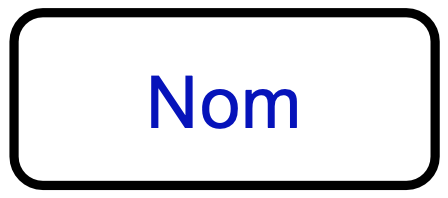
\includegraphics[scale=0.4]{./Images/Diagrammes/diagram_activite_elements_activite.png}
			\end{minipage}\\
		\cmidrule(lr){1-2}
			Activit\'e initiale & 
			\begin{minipage}[l]{0.3\textwidth}
				\centering
				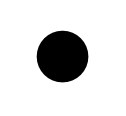
\includegraphics[scale=0.2]{./Images/Diagrammes/diagram_activite_elements_activite_initial.png}
			\end{minipage}\\
		\cmidrule(lr){1-2}
		Fin de flux & 
		\begin{minipage}[r]{0.3\textwidth}
			\centering
			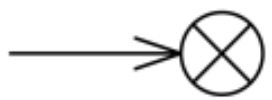
\includegraphics[scale=0.2]{./Images/Diagrammes/diagram_activite_elements_finflux.png}
		\end{minipage}\\
		\cmidrule(lr){1-2}
		Activit\'e finale & 
		\begin{minipage}[r]{0.3\textwidth}
			\centering
			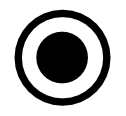
\includegraphics[scale=0.2]{./Images/Diagrammes/diagram_activite_elements_activite_final.png}
		\end{minipage}\\
	\cmidrule(lr){1-2}
	Flux de contr\^ole (transition) & 
	\begin{minipage}{0.2\textwidth}
		\centering
		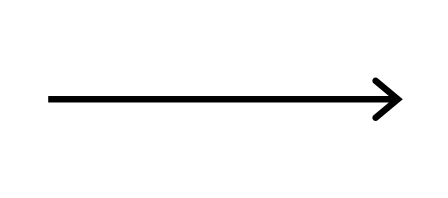
\includegraphics[width=\textwidth]{./Images/Diagrammes/diagram_activite_elements_fluxcommande.png}
	\end{minipage}\\
\cmidrule(lr){1-2}
Point de jonction (d\'ecision) & 
\begin{minipage}{0.5\textwidth}
	
\includegraphics[width=\textwidth]{./Images/Diagrammes/diagram_activite_elements_pointjonction.png}
\end{minipage}\\
\cmidrule(lr){1-2}
Barre de synchronisation & 
\begin{minipage}{0.5\textwidth}
	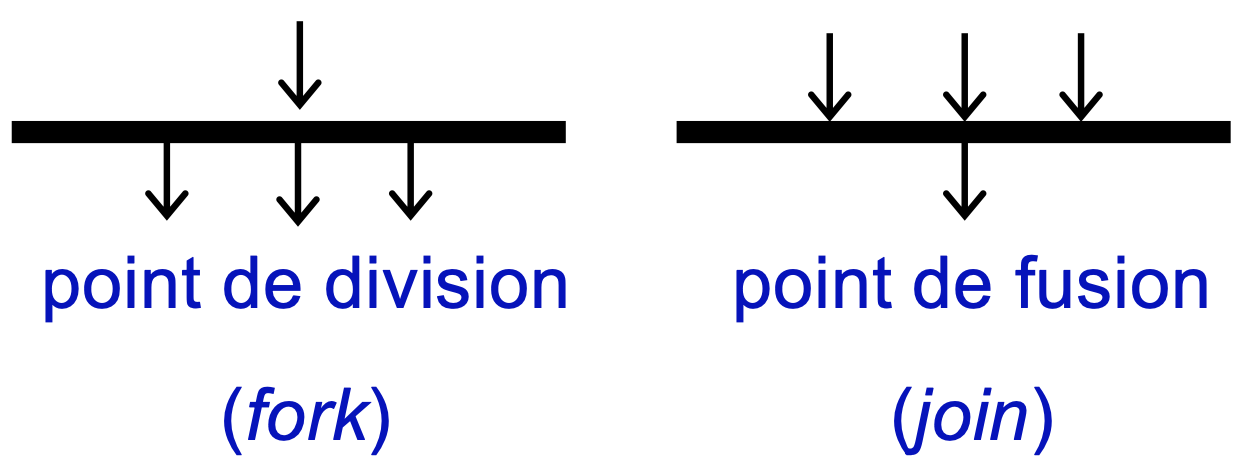
\includegraphics[width=\textwidth]{./Images/Diagrammes/diagram_activite_elements_barresynchro.png}
\end{minipage}\\
\cmidrule(lr){1-2}
Signaux & 
\begin{minipage}{0.5\textwidth}
	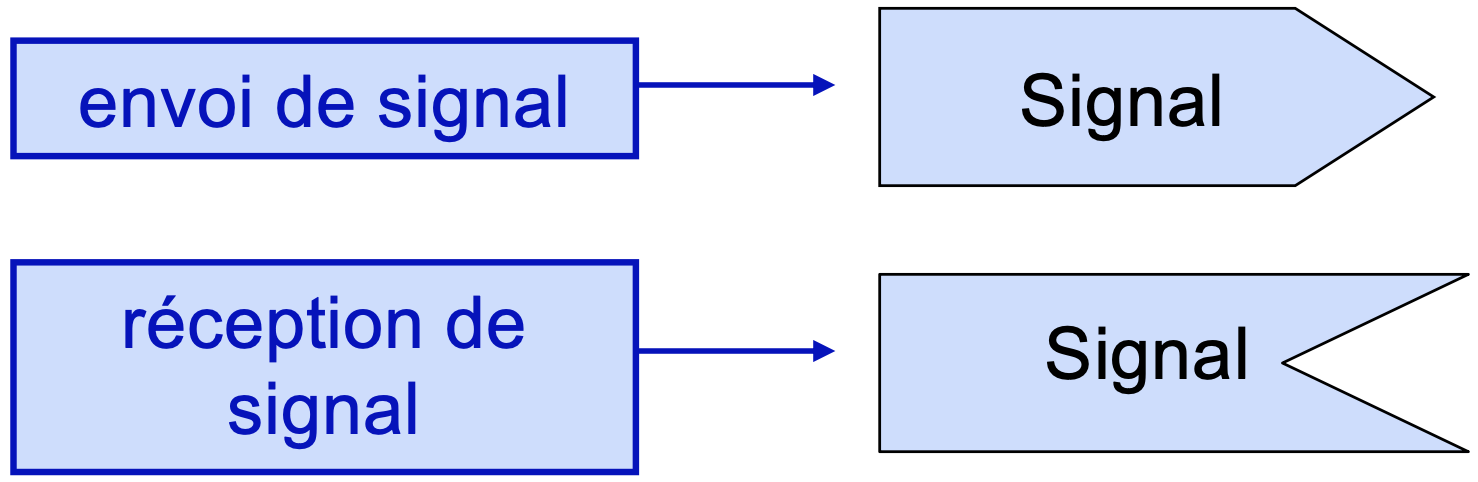
\includegraphics[width=\textwidth]{./Images/Diagrammes/diagram_activite_elements_signaux.png}
\end{minipage}\\
			\bottomrule
		\end{tabular}
	\end{adjustbox}
\end{table}


\begin{figure}[H]
	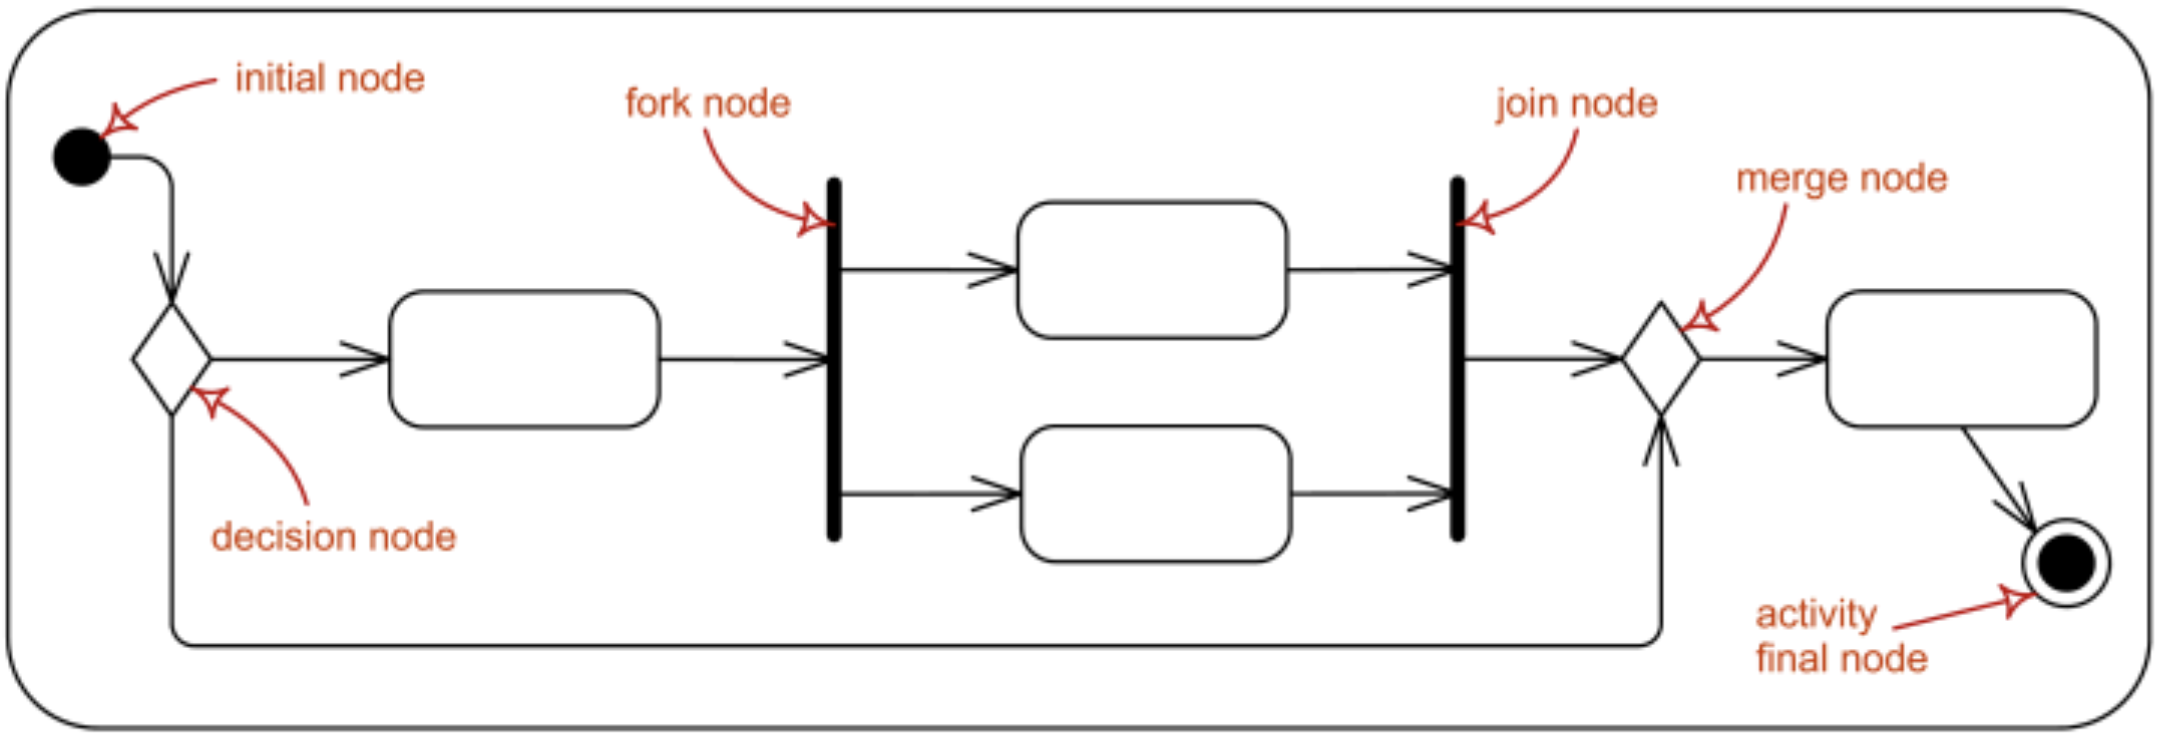
\includegraphics[width=\textwidth]{./Images/Diagrammes/diagram_activite_resume.png}
	\caption{R\'esum\'e d'un diagramme d'activit\'es.}
	\label{fig:diagram_activite_commente}
\end{figure}

\begin{figure}[H]
	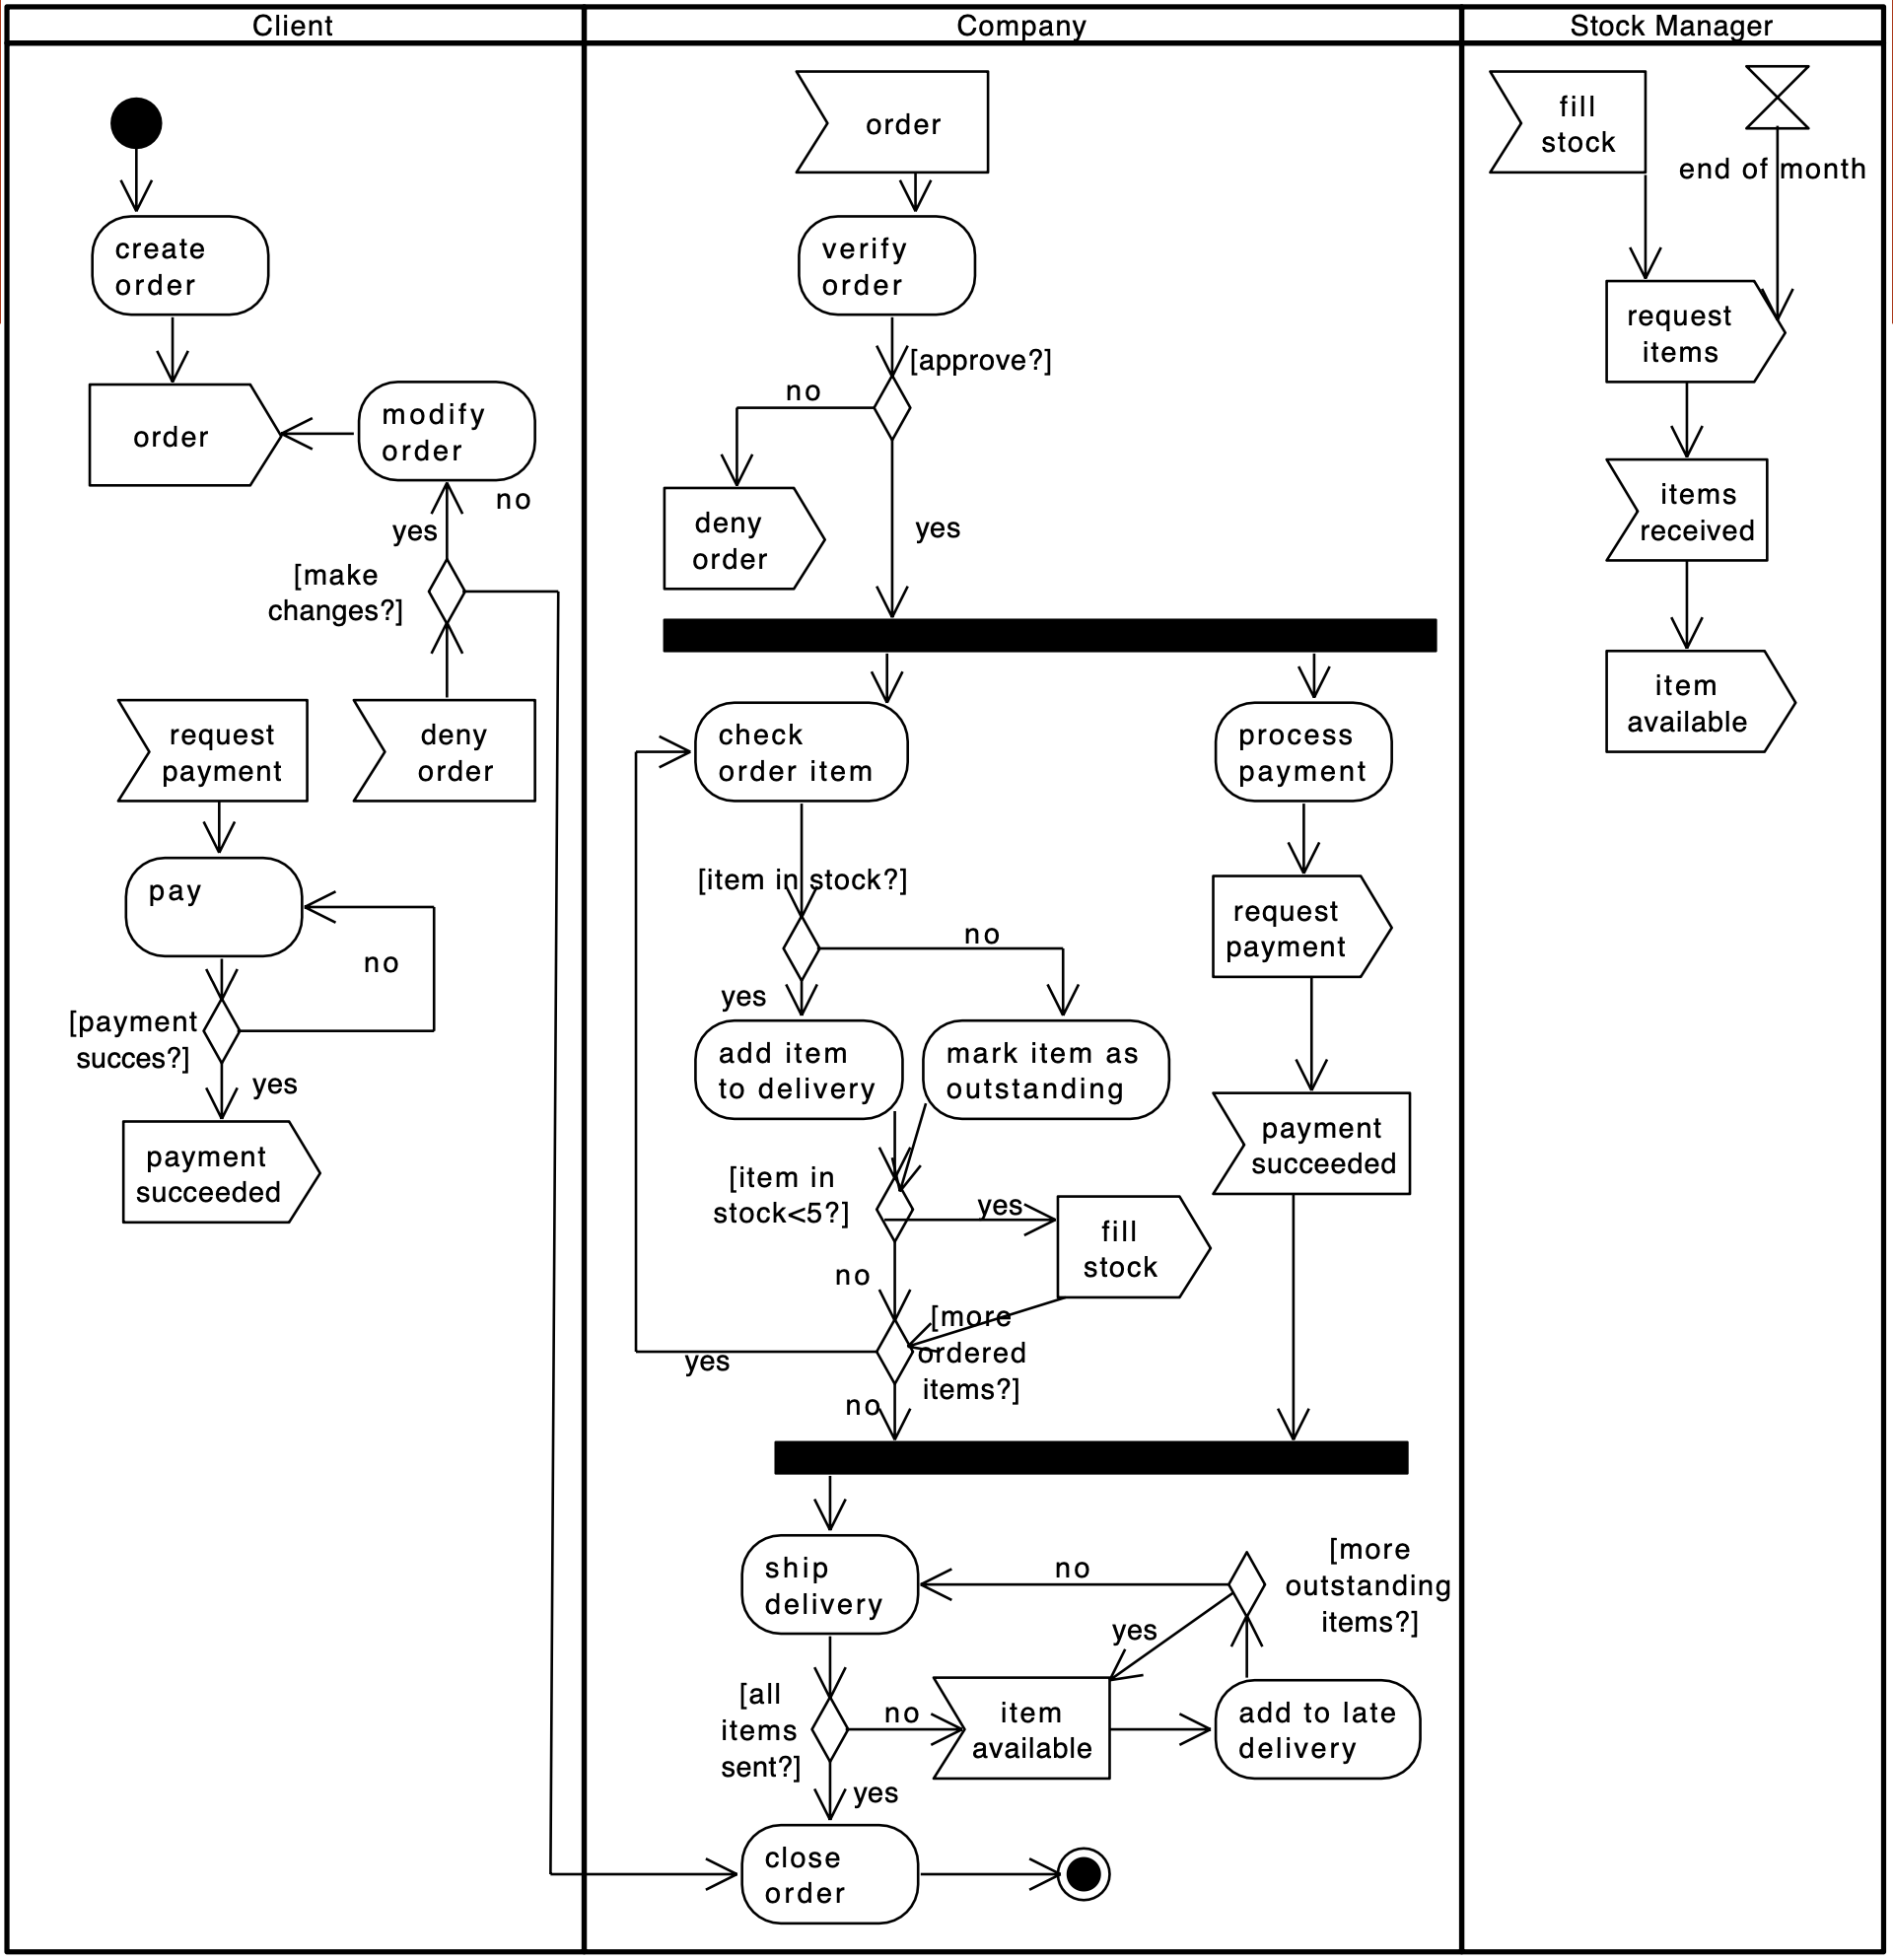
\includegraphics[width=\textwidth]{./Images/Diagrammes/diagram_activite_ex_complet.png}
	\caption{Diagramme d'Activit\'e : Exemple Complet.}
	\label{fig:diagram_activite_ex_complet}
\end{figure}


\newpage
